\documentclass[12pt]{article}
\usepackage[utf8]{inputenc}
\usepackage{graphicx}

\title{DD Lab 7 Assignment}
\author{Sai Kartik \\2020A3PS0435P}

\begin{document}
\maketitle
\section{T flip-flop using JK flip-flop}
\begin{center}
    \begin{figure}[ht]
        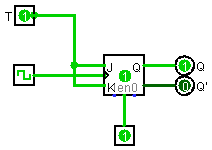
\includegraphics{twjk.png}
    \end{figure}
\end{center}
The truth table for the above circuit: \\[2ex]
\begin{tabular}{|c|c|c|c|c|}
    \hline
    J & K & T & $Q_n$ & $Q_{n+1}$ \\
    \hline
    0 & 0 & 0 & 0     & 0         \\
    1 & 1 & 1 & 0     & 1         \\
    1 & 1 & 1 & 1     & 0         \\
    0 & 0 & 0 & 1     & 1         \\
    \hline
\end{tabular}
\newpage
\section{JK flip-flop using D flip-flop}
\begin{center}
    \begin{figure}[ht]
        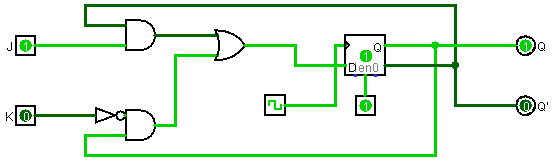
\includegraphics[scale=0.70]{jkwd.png}
    \end{figure}
\end{center}
The truth table for the above circuit: \\[2ex]
\begin{tabular}{|c|c|c|c|c|}
    \hline
    J & K & D & $Q_n$ & $Q_{n+1}$ \\
    \hline
    0 & x & 0 & 0     & 0         \\
    1 & x & 1 & 0     & 1         \\
    x & 1 & 0 & 1     & 0         \\
    x & 0 & 1 & 1     & 1         \\
    \hline
\end{tabular}
\end{document}